% ||||||||||||||||||||||||||||||||||||||||||||||
% Capitulo de Resultados Preliminares
% ||||||||||||||||||||||||||||||||||||||||||||||

\chapter{Análise de Resultados}

Neste capítulo são apresentados os resultados do projeto, os quais são os produtos dos estudos de casos desenvolvidos nas empresas parceira.
Como se trata de um estudo de caso, e para as empresas, uma prova de conceito, os resultados também foram divididos por equipamento avaliado:
exaustor e seladora. Os mesmo, inicialmente são apresentados capturas de telas do software na parte de análise dos sinais coletados, para fim
de dar uma visão global do estado de saúde do equipamento no dado momento. Na sequência, gráficos específicos, levantando características e 
comparações em diferentes condições, levantando a relação de causa e efeito. Por fim, apontamentos e discussões sobre os resultados de cada um
dos elementos, e também comparações entre os mesmos.

Para a apresetação dos resultados do exaustor, foram feitas capturas de tela do software do sistema que estava instalado no motor, de forma
remota e supervisionada pelos responsáveis pela manutenção dos mesmos. A figura \ref{fig:exaustor_1} é a captura de tela do sistema no dia
em que um relatatório sobre a saúde dos exautores foi gerado, com os dados daquele momento, e com os limites gerados pelo machine learning
no momento da instalação (06/12/2020).

As principais informações que podem ser vistas na captura de tela são: 

\begin{itemize}
    \item Configurações de visualização: campos para selecionar se o gráfico será em tempo real, ou os dados serão exibidos dentro de um
intervalo, além de permitir selecionar qual eixo se deseja visualizar;
    \item Configurações de de Alerta e Perigo: possui o botão para ativação e desativação do machine learning, além dos campos para se editar
os valores de alerta e perigo, conforme desejo do usuário;
    \item Gráfico de Velocidade RMS em $\SI{}{\milli\metre\per\second}$, que contém: reta da linha de base em azul escuro, dados de velocidade
amostrados em azul claro, linha da alerta em amarelo, e por fim, linha de perigo em vermelho;
    \item Gráfico de Pico de frequência da velocidade em $\SI{}{\hertz}$, que contém: dados do pico de frequência da velocidade amostrados em azul 
claro; 
    \item Gráfico de Velocidade RMS em $\SI{}{\milli\metre\per\second}$, que contém: reta da linha de base em azul escuro, dados de velocidade
amostrados em azul claro, linha da alerta em amarelo, e por fim, linha de perigo em vermelho;
    \item Gráfico de Temperatura em $\SI{}{\celsius}$, que contém: reta da linha de base em azul escuro, dados de temperatura
amostrados em azul claro, linha da alerta em amarelo, e por fim, linha de perigo em vermelho;
\end{itemize}

\begin{figure}[H]
    \caption{Captura de tela do sistema instalado no exaustor.}
    \begin{center}
        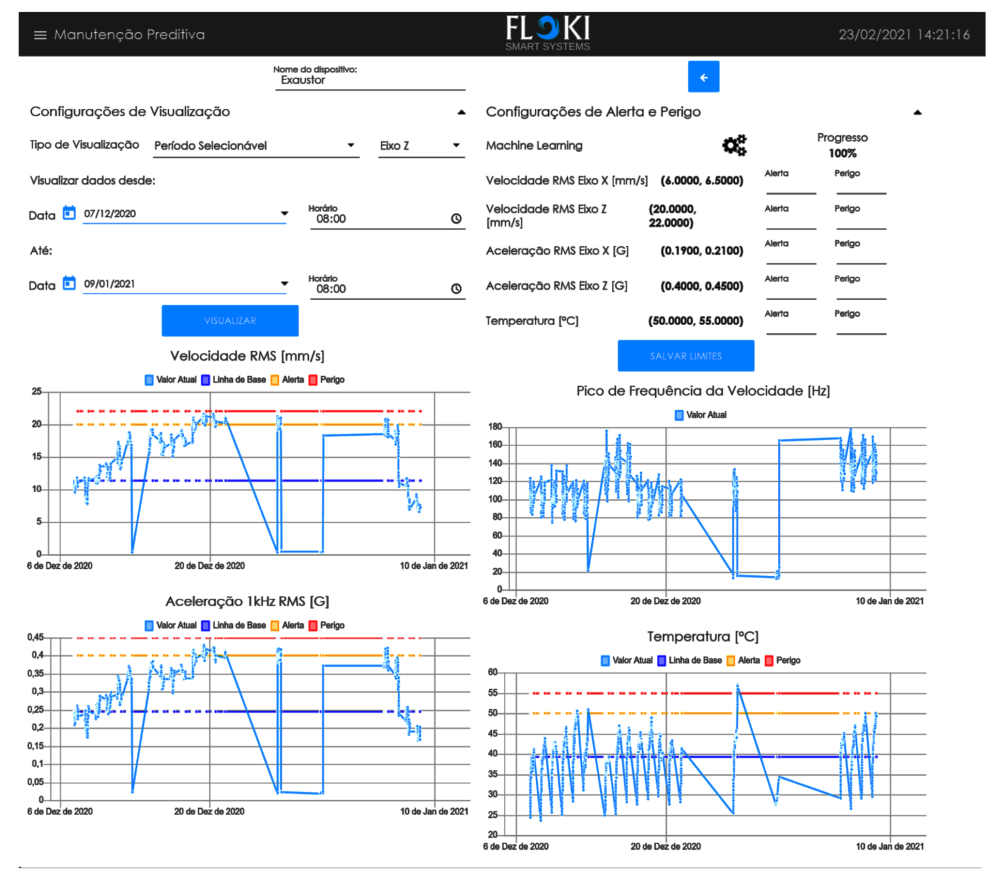
\includegraphics[scale=0.95, page=1]{resultados/img/resultados.pdf}
    \end{center}
    \fonte{Elaborado pelo Autor.} 
    \label{fig:exaustor_1}
\end{figure}

A captura de tela está com os dados de velocidade e aceleração do eixo x, como podemos ver. Fica claro que nenhuma das grandezas físicas
ultrapassam os limites estabelecidospelo machine learning, mas isso não significa que o motor esteja em bom estado. Se consultarmos a tabela 
\ref{tab:iso10816-1_randall_p146}, veremos que os valores para um motor de Classe I, segundo norma  ISO 10816-1, está entre apenas tolerável e
não permitido, dependendo do regime de funcionamento. Mas se olharmos o eixo z, que se encontra na figura \ref{fig:exaustor_xz}, os valores são
todos não permitidos, deixando claro o risco de falha eminente do motor.

\begin{figure}[H]
    \caption{Velocidade RMS [\SI{}{\milli\metre\per\second}] coletados do eixo x (A) e z (B).}
    \begin{center}
        \includegraphics[scale=0.55, page=2]{resultados/img/resultados.pdf}
    \end{center}
    \fonte{Elaborado pelo Autor.} 
    \label{fig:exaustor_xz}
\end{figure}

Como ficou claro, o eixo z se encontra em estado severo de vibração, não entrando em alarme devido ao machine learning tardio executado
pelo do operador, sendo agora uma tarefa mais de gestão do sistema, de se executar de forma mais adequada, que é logo após o recondicionamento 
ou ajustar manualmente os limites de acordocom a norma ISO 10816-1. Outra característica importante é a temperatura, quepode ser vista na figura
\ref{fig:exaustor_temperatura}, que teve uma dinâmica bem comportada e com característica de um sistema linear de primeira ordem.


\begin{figure}[H]
    \caption{Temperatura amostrada no exaustor.}
    \begin{center}
        \includegraphics[scale=0.65, page=3]{resultados/img/resultados.pdf}
    \end{center}
    \fonte{Elaborado pelo Autor.} 
    \label{fig:exaustor_temperatura}
\end{figure}

Fica nítido também o processo de aquecimento do dispositivo, seguindo os ciclos de funcionamento, que são bem regulares. O estudo de caso do 
exaustor se mostrou um ótimo caso para se analisar o comportamento do sistema em um dispositivo que já estava em funcionamento por um bom tempo 
após o recondicionamento, onde a técnica de machine learning, como esperado, não contribuiu com o objetivo de se detectar falhas, pois as
condições iniciais não eram as ideais e os limites ficaram além dos permitidos. Mas o funcionamento geral da ferramenta foi excelente, sem nenhum
problema grave reportado, funcionando dentro das especificações e dentro do esperado pela empresa parceira. Um relatório foi gerado e entregue
para a empresa, contendo todos os dados e explicações, o qual foi aceito e gerou uma ordem de compra da aplicação.

A segunda prova de conceito foi realizada em uma seladora, como descrito anteriormente, onde 5 sensores foram distribuídos pela máquina, com o 
objetivo de monitorar os pontos críticos. Esta máquina não apresenta um processo tão contínuo como o exaustor, exigindo uma amostragem maior
para se captar todas as características do funcionamento. Como no caso do exaustor, foram relaizadas capturas de telas do sistema, onde a figura
\ref{fig:seladora} representa a captura dos dados do sensor 5, 4 dias antes de uma falha (08/12/2020). Estes sensores foram instalados no dia 
13/11/2020, mas  os dados começaram a ser amostrados apenas no dia 16/11/2020, onde a ferramenta de machine learning fui usada e limites foram 
criados. 

\begin{figure}[H]
    \caption{Linhas de base e sinais coletados em um dos 5 sensores na Seladora.}
    \begin{center}
        \includegraphics[scale=0.95, page=4]{resultados/img/resultados.pdf}
    \end{center}
    \fonte{Elaborado pelo Autor.} 
    \label{fig:seladora}
\end{figure}



\begin{figure}[H]
    \caption{Linhas de base e dados de velocidade [\SI{}{\milli\metre\per\second} no momento da instalação
    (16/11/2020) x próximo da falha (4/12/20).}
    \begin{center}
        \includegraphics[scale=0.55, page=5]{resultados/img/resultados.pdf}
    \end{center}
    \fonte{Elaborado pelo Autor.} 
    \label{fig:seladora_antes_depois}
\end{figure}


\begin{figure}[H]
    \caption{Temperatura [\SI{}{\celsius}] amostrada na seladora.}
    \begin{center}
        \includegraphics[scale=0.8, page=6]{resultados/img/resultados.pdf}
    \end{center}
    \fonte{Elaborado pelo Autor.} 
    \label{fig:seladora_temperatura}
\end{figure}



Após a escrita de todo o trabalho, indo desde o conhecimento mínimo para o entendimento das propostas, passando pela descrição dos métodos
empregados, até os resultados preliminares, foi possível ver o funcionamento satisfatório das técnicas, mas que ainda precisam de melhorias
e a aplicação de uma CNN para classificar os resultados até agora obtidos. 